\subsection{Out-of-Distribution Detection}
Early studies on outlier detection often adopt unsupervised clustering methods to detect malformed data~\citep{DBLP:journals/air/HodgeA04, chandola2009anomaly,zimek2012survey}. In recent years, a substantial body of work has been directed towards improving the generalization capacity of machine learning models on out-of-distribution (OOD) data~\citep{DBLP:journals/pieee/RuffKVMSKDM21, hendrycks2020many}. 
\citet{DBLP:conf/iclr/HendrycksG17} find that simple statistics derived from the outputting softmax probabilities of deep neural networks can be helpful for detecting OOD samples. Following this work, \citet{dcbe7abf4db64d1b89bf9802585660ed} propose to use temperature scaling and add small perturbation to input images to enlarge the gap between in-scope and OOD samples. 
\citet{lee2017training} propose to add a Kullback-Leibler divergence term in the loss function to encourage assigning lower maximum scores to OOD data. 
% \citet{lee2017training} used GAN~\citep{goodfellow2014generative} to detect out-of-scope images. Specifically, the discriminator in GAN is trained to produce low confidence scores for the out-of-scope samples.

Recently, there is a line of work that employs synthetic or real-world auxiliary datasets to provide learning signals for improving model robustness under various forms of distribution shift~\citep{DBLP:journals/corr/GoodfellowSS14,DBLP:journals/corr/abs-1907-07640,DBLP:conf/icml/HendrycksLM19,lee2017training}. Particularly, \citet{hendrycks2018deep} propose to leverage large-scale public datasets to represent outliers during training time and form a regularization term based on that. This idea is similar to our proposal of constructing open-domain outliers, but we use a simpler, end-to-end, $(K+1)$-way discriminative training procedure without any regularization term or threshold parameter.  

\begin{figure*}[t]
    \centering
    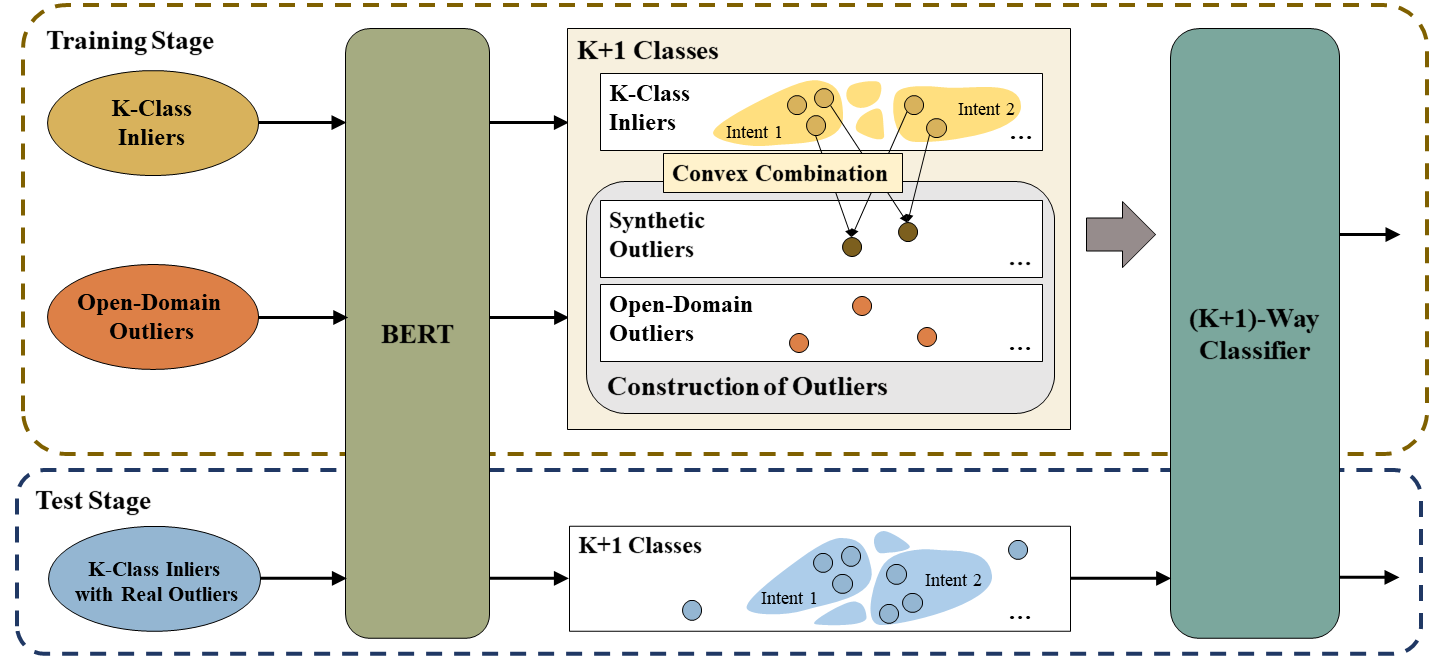
\includegraphics[width=150mm]{framework.png}
    \caption{An illustration of our proposed method. We use BERT as the utterance encoder. At training stage, we train a (K+1)-way classifier by constructing two types of pseudo outliers. The open-domain outliers are collected from an auxiliary dataset disjoint from both the training and test data. The synthetic self-supervised outliers are generated during training by random convex combinations of features of inliers from different known classes.}
    \label{fig:framework}
\end{figure*}
\subsection{Out-of-Scope Intent Detection}
While \citet{DBLP:conf/acl/HendrycksLWDKS20} find that pretrained transformer-based models like BERT are intrinsically more robust to OOD data, they suggest that there are still margins for improvement. Therefore, we build our model on top of BERT to improve intent detection under significant distribution shift. Previous methods for out-of-scope (or out-of-distribution) intent detection are commonly threshold-based, where models output a decision score and then compare it with a threshold that is predefined or selected by cross-validation. 

There are mainly three branches of related work. The first group uses a confidence score which determines the likelihood of an utterance being out-of-scope. 
For example, \citet{DBLP:conf/emnlp/ShuXL17} build $m$ binary Sigmoid classifiers for $m$ known classes respectively and select a threshold to reject OOD inputs that may have lower probabilities than the threshold across all $m$ classifiers. 
Similar to the OOD data generation method used in \citet{lee2017training}, \citet{ryu-etal-2018-domain} employ GAN~\citep{goodfellow2014generative} to generate simulated OOD examples with the generator and learn to reject simulated OOD examples with the discriminator.

The second group identifies out-of-scope sentences through reconstruction loss. For example, \citet{10.1016/j.patrec.2017.01.008} build an autoencoder to encode and decode in-scope utterances and obtain reconstruction loss by comparing input embeddings with decoded ones. Out-of-scope utterances result in higher reconstruction loss. 

The third group leverages off-the-shell outlier detection algorithms such as local outlier factor (LOF)~\citep{10.1145/335191.335388}, one-class SVM~\citep{6790022}, robust covariance estimators~\citep{article}, and isolation forest~\citep{10.1109/ICDM.2008.17} to detect out-of-scope examples. Utterance embeddings belonging to a specific class will be mapped to the corresponding cluster (usually modeled by a Gaussian distribution) while out-of-scope samples will be pushed away from all in-scope clusters. Examples of this kind include SEG~\citep{DBLP:conf/acl/YanFLLZWL20} and LMCL~\citep{DBLP:conf/acl/LinX19}. Very recently, \citet{Zhang_Xu_Lin_2021} propose to learn adaptive decision boundaries after pre-training instead of using off-the-shell outlier detection algorithms.
% in which they varied in methods to extract the sentence embedding.

In addition, some other work focuses on out-of-scope detection in few-shot scenarios. \citet{tan-etal-2019-domain} leverage independent source datasets as simulated OOD examples to form a hinge loss term. \citet{zhang-etal-2020-discriminative} propose to pretrain BERT by a natual language understanding task with large-scale training data to transfer useful information for few-shot intent detection. 

Finally, for our proposal of constructing synthetic outliers, the most similar method is {Mixup} proposed by \citet{DBLP:conf/iclr/ZhangCDL18}. However, their method is designed for data augmentation to enhance in-distribution performance and requires corresponding combinations in the label space \cite{DBLP:conf/nips/ThulasidasanCBB19}.

%which is essentially important as suggested by


% OOS in general:  
% Neural Network Based: MSP, Variational AutoEncoder, DOC, ODIN (CV).


% OOS in NLP: SEG, LMCL, VAGAN, Word Graph EMbedding, GAN-based, GDA + Mahalanobis distance, OOD for Low Resource. , AutoEncoder, Variational AutoEncoder



% Some defined Outlier Detection problem as binary classification problem. (AutoEncoder)
% Assumption: Open word / Close word Assumption


% Out-of-Domain Detection/Anomaly Detection/ Novelty Detection/ Out of Distribution Detection
%Category: (1) Reconstruction Loss; (2) Confidence Base (3) Outlier Detection / Distance Base
% Previous Studies:  GAN base (2) / Auto Encoder (1) / Variational Auto Encoder (1) / VAGAN (1) / LMCL (3) / SEG  (3) / ADB (3) / ODIN(2)/  MSP(2) / Word Graph Embedding (2) / DOC(
% Intent Classification: Associate utterance to intent, commonly by probability after Softmax
% Category (2) Set up a threshold and compare to the highest probability class. [MSP, ODIN(MSP with temperature scaling)]
% Category (1) Auto Encoder Base: Encode sentence embedding to a smaller hidden space and reconstruct it. Outlier sample produce higher reconstruction loss.  [Auto Encoder; Variational Auto Encoder; VAGAN]
% Category (3) Clustering Base; Treat OOS as outlier detection problem. [LMCL; SEG; ADB] 

%Intent classification has been broadly used by many dialog systems such as chat-bot with the task of predicting input utterance into one of the intents. Most of the studies focus on closed word assumption where no new intent will appears during testing. Traditional intent classification model classify utterance by using Soft-max activation function to acquire probability for each intent and output intent with highest probability. However, it is also critical to  detect out of  scope utterance as they will inevitably appears in dialog systems. With the capability to detect out of scope sentence, developers will be able to identify potential improvement and improve the flexibility of their dialog system.